\documentclass[]{article}
\usepackage[a4paper]{geometry}
\usepackage{multicol}

\usepackage{cite}
\usepackage{hyperref}
\usepackage{caption}
\usepackage{graphicx}
\graphicspath{{./images/}}
\newenvironment{Figure}
{\par\medskip\noindent\minipage{\linewidth}}
{\endminipage\par\medskip}

\usepackage{dsfont}

\title{Deep Learning Fall 2019 Project Report\\\large{Memory Limitations and Non-Trainable Parameters}}
\author{Bram van den Heuvel \& Matej Sladek}

\pagestyle{empty}

\begin{document}

\maketitle

\begin{abstract}
	We realize that an arbitrary number of non-trainable weights can be represented by a (single) seed. We propose a memory saving technique for non-trainable parameters that recomputes weights during training and evaluation in a way that incurs a "lower than naively expected" runtime cost. We then attempt to utilize large numbers of non-trainable weights in various architectures and report on the model performance. Our experiments generally showed that performance doesn't improve when adding more non-trainable weights to an architecture while training stability was improved in one classification task.
\end{abstract}


\begin{multicols}{2}
	\section{Introduction}\label{introduction}
	Classical statistics suggests there is a paradox going on in deep learning: the models have an enormous number of parameters, but they do not suffer from the downsides of that fact the same way that virtually all other model classes do.
	
	In the early 1990's, Schmidt et. al. \cite{Schmidt_Kraaijveld_Duin} attempted to explain this phenomena by showing that many of the parameters in a deep model are of less importance. They describe how the first layers of a neural net can be viewed as a collection of nonlinear features of the input data, with a simple linear regression attached to it in the final layer. The weights in the final layer are of higher importance. They demonstrate this by randomly initializing some of the hidden layers with random weights and keeping their values fixed throughout the training procedure. We call these layers \emph{random layers}. The training procedure still works surprisingly well.
	
	The value of depth and a large number of parameters is demonstrated by the models performing best in the ImageNet Large Scale Visual Recognition Challenge (INLSVRC) \cite{DBLP:journals/corr/CanzianiPC16}. In the last decade, the number of layers in the top-performing model has gone up to 152 with ResNet. Also the number parameters has grown; models often use tens of millions of parameters, VGG-19 as much as 155 million. This translates to a maximum memory usage during training of approximately 200 MB for most models, a little over 800 MB for VGG-19, when trained with a batch size of one. This then increases to above 1000 MB for several top-performing models once the batch is increased to 16, and increases approximately linearly with batch size beyond that \cite{DBLP:journals/corr/CanzianiPC16}.
	
	This means that with a batch size of 64, none of the top performing models can be trained on a mobile device or a consumer-grade GPU because of memory limitations. When we consider memory limited mobile devices, even model evaluation is challenging. In that case, the vast majority of memory is required for the trained weights (as activations don't need to be remembered). With memory scheduling, memory requirements can be reduced greatly, but at a run-time cost \cite{Li_Shen_Dou_Ni_Xu_Yang_Wang_Niu_2019} presumably due to memory bandwidth and latency limitations.
	
	We attempt to improve on the memory / performance / time trade-off by utilizing non-trainable parameters to improve architectures with few trainable parameters. We start by introducing a training and evaluation technique in section \ref{recomputation} that allows for training and evaluation models with a large amount of non-trainable parameters quickly. We then experiment with such architectures in section \ref{experiments}.
	
	\section{Recomputation}\label{recomputation}
	We realize that an arbitrary number of non-trainable parameters can be represented by a (single) seed. A Pseudo Random Number Generator (PRNG) can generate values that are "hard to distinguish" from independent realizations of a certain distribution. They typically work sequentially, or in the case of multiple threads, one seed per thread is used if the values need to be generated reproducibly. These methods are sufficient to save on model storage costs for large models.
	
	A more realistic problem is memory usage during training, as was made clear in section \ref{introduction}. The memory usage typically peaks at the end of the forward pass, when the model weights and the activations are stored in memory. Recomputation of activations during the backward pass, by only saving a subset of the computed activations and recomputing them from the last layer they are known from, allows for sub-linear maximum memory usage in the number of layers during training \cite{chen2016training}. See \cite{DBLP:journals/corr/GruslysMDLG16} for an algorithm specialized for recurrent models.
	
	While one typically recomputes a majority of the activations with the algorithm in \cite{chen2016training}, the runtime increase is shown to be only 30\% for a 4x reduction in maximum memory usage when training an LSTM under a long sequence unrolling setting. It is hypothesized that this can be explained in part by the under utilization of computational resources in a GPU, where memory bandwidth is often a limiting factor\footnote{We found no scientific research on this (engineering) subject, but plenty of anecdotal evidence in blog posts such as these: \url{https://nestlogic.com/index.php/2019/02/11/gpu-utilization-with-neural-networks/} and  \url{https://towardsdatascience.com/measuring-actual-gpu-usage-for-deep-learning-training-e2bf3654bcfd}} (a simple improvement would be to increase the batch size, but this directly increases the maximum memory usage as explained in section \ref{introduction}).
	
	If an architecture contains many non-trainable parameters, a Pseudo Random Function (PRF) \cite{Goldreich_Goldwasser_Micali_1986} can be utilized to regenerate these during training also. Now, it is not only the activations that one (partially) recomputes, but \emph{some of the network's weights as well}. PRFs can be viewed as PRNG's which don't generate values $(v_1, v_2, \ldots)$ in sequence, but instead can evaluate in constant time a function $\mathds{N} \ni n \mapsto v_n$. They stem from cryptography and the well-known ones are made for such applications, unsuitable for training neural networks. The requirements for a pseudo random function are different for this application: speed and memory usage matter, the quality of the generated numbers less. For a sketch of a first idea of a pseudo random function for this application, see the appendix. The memory requirements of such a function are low enough to evaluate it using register memory only and without any communication with memory or across cores. In this way, there is no memory access incurred for non-trainable weights, which we think will be reflected favorably in the training time of these models: GPU's can have memory limitations, such as the TitanX GPU, which has only approximately 1KB of per-thread memory that can be read from fast enough to saturate the floating point datapath \cite{DBLP:conf/icml/DiamosSCCCEEHS16}. 
	
	Note that these benefits apply during both training and evaluation.
	
	\section{Experiments}\label{experiments}
	The scope and duration of this project didn't allow for an actual implementation of a PRF, computed within the GPU core. We couldn't actually test many of the training- and evaluation time influencing aspects mentioned above. It however did provide a motivation to explore how the usage of non-trainable parameters could improve the performance of models with few trainable parameters.
	
	\subsection{Choosing benchmark problems}
	We attempt to find model architectures that utilize untrainable parameters while performing well. To that end we introduce new random layers, or replacing existing layers by random layers on different baseline architectures. We measure model performance exactly by simply storing the random layers completely. In all our experiments, the number of trainable parameters grows very slowly, or not at all, in comparison to the number of non-trainable parameters we add.
	
	Some of the tasks we selected while writing our proposal turned out to be too easy to solve (MNIST \cite{lecun-mnist}) or improvements too hard to measure without long evaluation times (Higgs dataset \cite{Dua:2019}), and any improvements therefor hard to measure. We identified the following more difficult tasks:
	\begin{itemize}
		\itemsep0em
		\item Convolutional architecture to classify images from the MNIST fashion dataset \cite{xiao2017/online}
		\item Dense architecture to classify level of income on the census income dataset, classifying income \cite{Asuncion+Newman:2007}
		\item Dense architecture to do regression on the census income dataset, predicting age \cite{Asuncion+Newman:2007}
	\end{itemize}
	For the census income dataset, a label embedding was used.
	
	We chose to not work with two model sizes (small and large) for each task as planned, we had trouble to find situations in which adding non-trainable parameters was beneficial at all and as such did not find suitable baseline models. Different tests turned out to be suitable for different tasks.
	
	We then take a slightly different approach, and use Bayesian optimization to find good hyperparameters with a constraint on the number of trainable parameters, as all others could be regenerated as described in section \ref{recomputation}.
	
	We use maximum likelihood loss for classification and squared error for regression loss for regression tasks. For all training, the Adam optimizer was used with an early stopping callback. We evaluate using accuracy for classification and squared error for regression.
	
	\subsection{Results}\label{results}
	\subsubsection*{Task 1: Convolutional architecture for classification}
	The convolutional models demonstrated stable performance and were not cross validated. For all architectures, we started with 32 trainable convolutions of shape (3, 3) with no strides and ReLU activations, followed by a (2, 2) maxpool with strides of (2, 2) and a flatten. We used at least a trainable dense layer with a softmax activation at the end. The baseline model contains the layers mentioned in this paragraph and nothing else.
	
	We were unable to see any benefit from adding random layers. We did expect to find some improvement: in another ETH lecture, attended by one of the team members, it was demonstrated on MNIST that the baseline model with a single trainable layer of size 128 added performs at 98\% accuracy after a single epoch. Setting that extra layer as untrainable lead to an accuracy of 91\%. The implication in that lecture was that random layer was useful although it had no learnable parameters itself. I.e. it is better to learn from a large number of random features of the previous layer, than it is to learn from the previous layer itself. Our experiments however show that this is not true; the model performs equally well or better without the extra random layer added, which was not tested during that lecture.
	
	\subsubsection*{Task 2: Dense architecture for classification}
	We now use 10-fold CV to be able to assess smaller differences in performance. All architectures consist only of fully connected layers, with random layers in the middle of the network. We do a grid search, varying over different aspects of the architecture (whether there is a trainable layer before the random layers, how many random layers there are and of which size, whether there is a trainable layer after the random layers and before the trainable outputlayer with softmax activation). We notice that there are some configurations in which the model training is unstable without a random layer. Then, either the training is successful or not, with the random layer not improving performance in the first case. We were unable to explain why the training stability improved. The scores are visualized in figure \ref{fig:average_classification}.
	
	\begin{Figure}
		\centering
		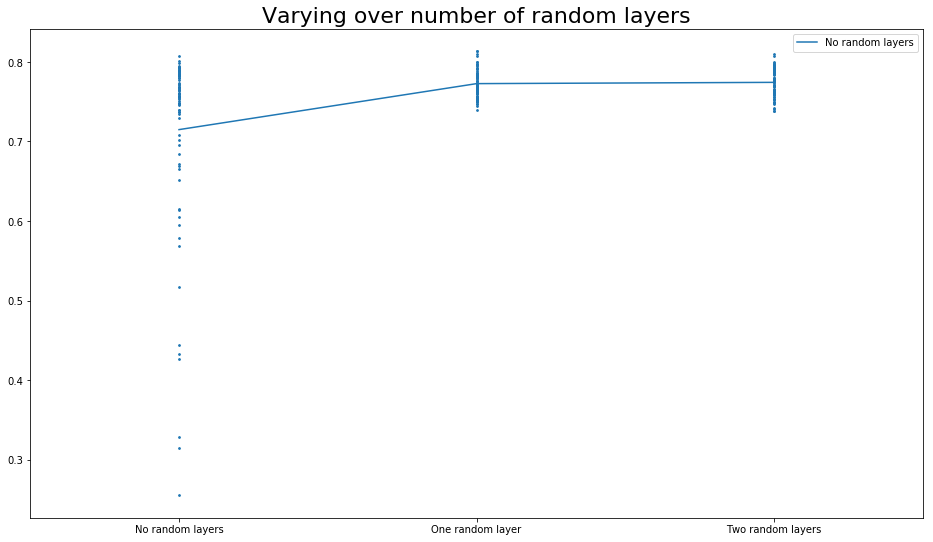
\includegraphics[width=\linewidth]{average_classification}
		\captionof{figure}{Census income dataset classification accuracy: stability improvement.}
		\label{fig:average_classification}
	\end{Figure}
	
	\begin{Figure}
		\centering
		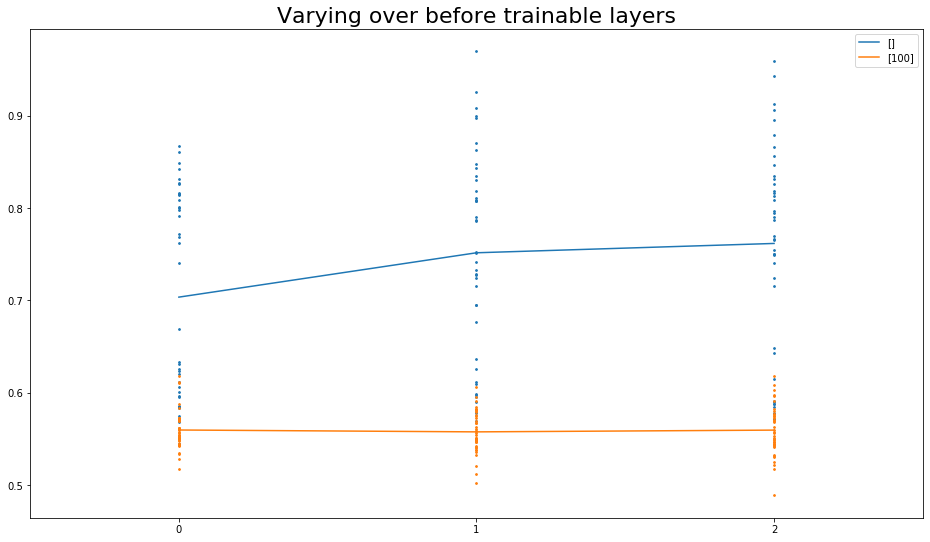
\includegraphics[width=\linewidth]{average_regression}
		\captionof{figure}{Census income dataset regression score: no weights per layer.}
		\label{fig:average_regression}
	\end{Figure}
	
	\begin{Figure}
		\centering
		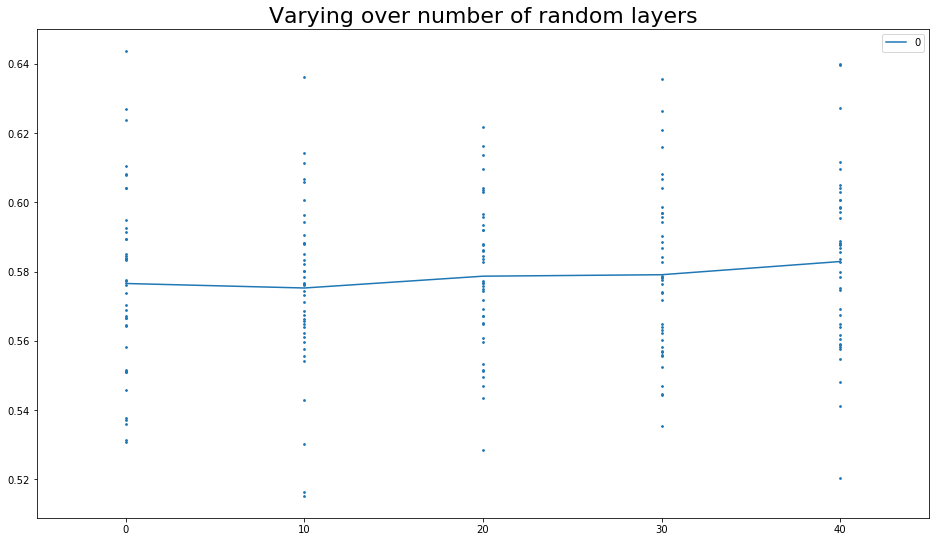
\includegraphics[width=\linewidth]{average_regression_residual}
		\captionof{figure}{Census income dataset regression score: residual network, one weight per layer. Averages split out on whether there is a trainable layer of size 100 at the start.}
		\label{fig:average_regression_residual}
	\end{Figure}
	
	\begin{Figure}
		\centering
		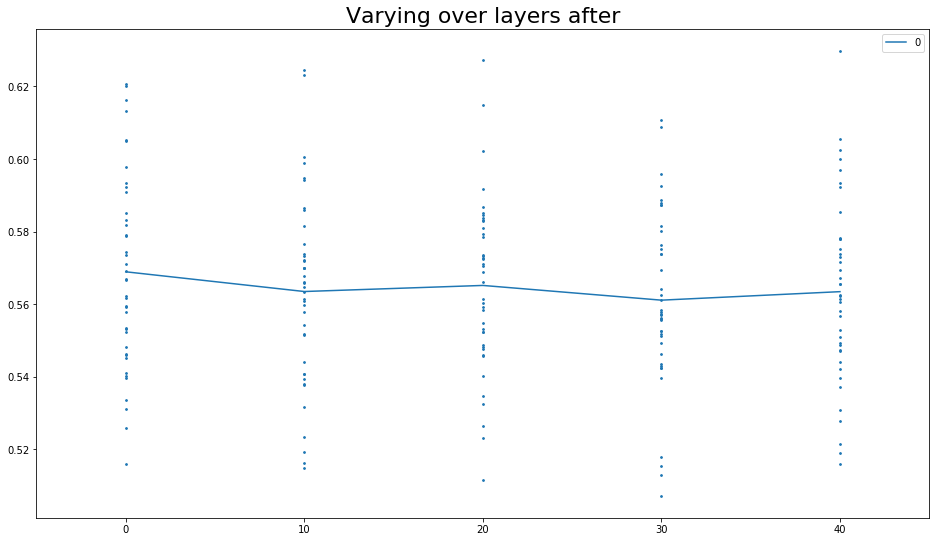
\includegraphics[width=\linewidth]{average_regression_residual_node}
		\captionof{figure}{Census income dataset regression score: residual network, one weight per node}
		\label{fig:average_regression_residual_node}
	\end{Figure}
	
	\subsubsection*{Task 3: Dense architecture for regression}
	Again we use 10-fold CV, and first the architectures are the same as in Task 2. We trained a random forest for reference, which performs with a loss of about .42 before hyperparameter tuning. The results are displayed in figure \ref{fig:average_regression}. For these architectures, the number of trainable parameters stays constant as more random layers are added. We now change our architecture to a residual one, with a single trainable parameter controlling the magnitude of the change per layer. With the number of trainable parameters now growing linearly with the number of layers, performance now doesn't noticably change as we add more layers, as can be seen in figure \ref{fig:average_regression_residual}. We used linear, $\tanh$ and relu activations with similar results. We now modify the last experiment one step further, and use a single trainable parameter not per layer but per node. Each weight controls how much of the random map, applied to the values of the last layer, gets added to each coordinate of our state vector as the data flows through the network. For the first time now, the performance increases (albeit slowly) as more layers get added. See figure \ref{fig:average_regression_residual_node}.
	
	\subsubsection*{Automated architecture optimization}
	We try to utilize an increased number of non-trainable parameters to increase the performance per trainable parameter. In our experiments, performance increased only with an increase in layers when a certain minimum number of trainable parameters per layer was included in the architecture (compare figure \ref{fig:average_regression_residual} with figure \ref{fig:average_regression_residual_node}). That gives rise to the question, whether trainable parameters are best used with, or without non-trainable parameters in the mix. We did an automated hyperparameter search using Bayesian optimization, allowing the algorithm to allocate trainable weights to trainable dense layers and random layers with one scalar per node.
	
	The regression problem of task 3 is used. The possible architectures were as follows. There is always a relu activated random layer at the start, of varying size. Then come zero or more random residual layers, with one weight per node. These are followed by an optional trainable layer of varying size before a final trainable dense layer. Untrainable batch normalization can be enabled. All activations are relu. The total number of trainable weights is less or equal to 100.
	
	Bayesian optimization finds that a large random layer at the start (30-47), followed by no random layers and a trainable layer of size two or three before the final regression is optimal. Batch normalization is rarely enabled in a good set of hyperparameters.
	
	\section{Discussion}
	Except for an improvement in training stability for a specific task and architecture, we found no way to utilize large amounts of non-trainable parameters to improve models with few trainable parameters. Especially the automated architecture optimization results demonstrate that the trainable parameters are best allocated in classical trainable layers, rather than choosing how much of random maps to apply in residual layers. Naturally, it is always possible to consider more configuration in which non-trainable parameters could be utilized, but we don't have any specific architectures in mind that we would like to try next.
	
	\section{Summary}
	We attempted to improve on the memory / performance / time trade-off by utilizing non-trainable parameters to improve architectures with few trainable parameters. While there are a lot of (engineering) reasons to believe that enormous models could be trained and evaluated with very little memory and a "better than naively expected" time penalty, these architectures didn't outperform architectures with no or few non-trainable parameters in our experiments.
	
	\appendix
	\section*{Appendix: Possible pseudo random function for neural networks}
	We choose a simple hash function $h$, to be evaluated on a tuple of
	\begin{enumerate}
		\itemsep0em
		\item a unique identifier for layer and
		\item the coordinates of the parameter.
	\end{enumerate}
	The resulting bits are then interpreted as a float in $[0, 1]$ to be used as input of the inverse of a cumulative distribution function.
	
	The above is merely a first idea from non-experts. For more idea's in this 'hash function direction', see for example \cite{TAOCP364} or \cite{wiki:Hash_function}.

	\bibliography{../bibliography}
	\bibliographystyle{plain}
\end{multicols}

\end{document}
